%!TEX root = Manuscript.tex

\chapter{Comparison of precise matching on DSMs and original RGB images}
\label{chap:appendix4}
In order to decide which type of images (DSMs or original images) is more suitable for executing the precise matching, we apply our pipeline \textit{Patch} on both DSMs and original images of Fr{\'e}jus 1970 and 2014.
The final matches are displayed in Figure~\ref{precisematchingdepth} (a) and (b). 
To asses quantitatively the results, we created a GT depth map and calculated the accuracy (correct matches / total matches). In Figure~\ref{precisematchingdepth}~(c) we plot the accuracy curves while varying the reprojection error threshold from 0 to 10 pixels. 
{It is clear that} the result using the original images is more accurate, even though the DSMs recovered more correspondences.
This is because historical DSMs at full resolution are too noisy to guarantee high precision measurements (see the DSM shaded image in Figure~\ref{precisematchingdepth} (d).
\begin{figure*}[htbp]
	\begin{center}
		\subfigure[Matches on RGB images]{
			\begin{minipage}[t]{0.48\linewidth}
				\centering
				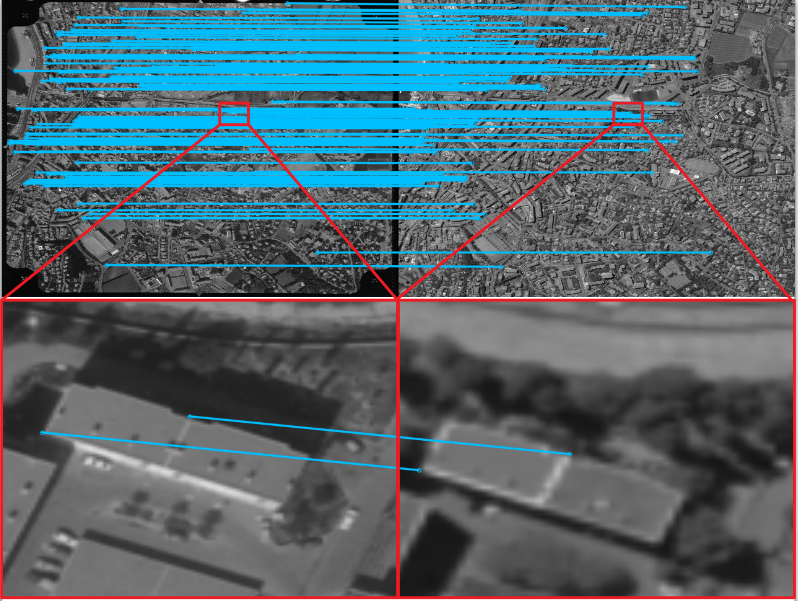
\includegraphics[width=6cm]{images/appendix4/TiePtOriImg.png}
				%\caption{DoD$_{Pezenas\_1971}^{Co-Reg}$}
			\end{minipage}%
		}
		\subfigure[Matches on DSMs]{
			\begin{minipage}[t]{0.48\linewidth}
				\centering
				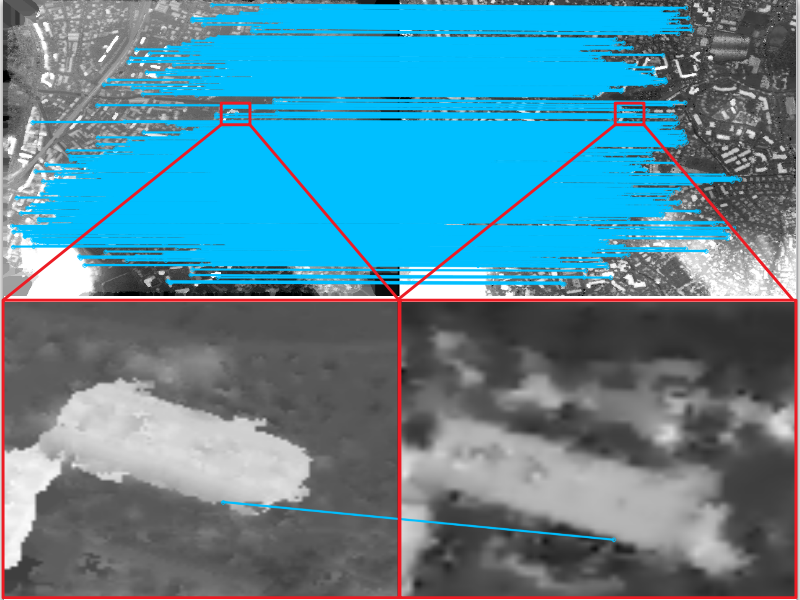
\includegraphics[width=6cm]{images/appendix4/TiePtDepth.png}
				%\caption{DoD$_{Pezenas\_1971}^{Guided}$}
			\end{minipage}  
		}       
		\subfigure[Accuracy of (a) and (b)]{
			\begin{minipage}[t]{0.58\linewidth}
				\centering
				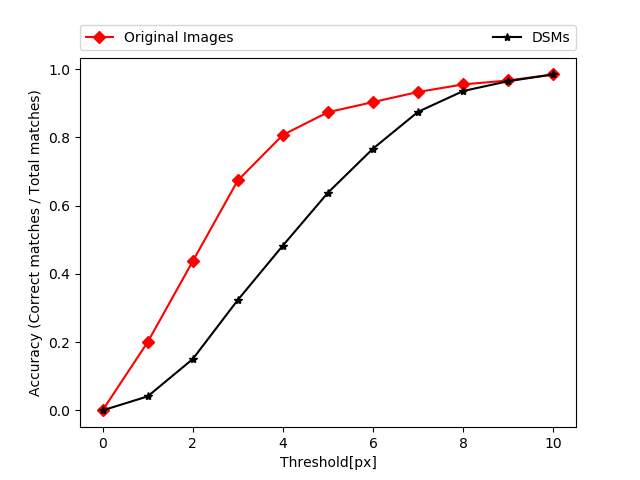
\includegraphics[width=7cm]{images/appendix4/pdfdepth.png}
				%\caption{DoD$_{Pezenas\_1981}^{Co-Reg}$}
			\end{minipage}%
		}
		\subfigure[Shaded image of historical DSM]{
			\begin{minipage}[t]{0.38\linewidth}
				\centering
				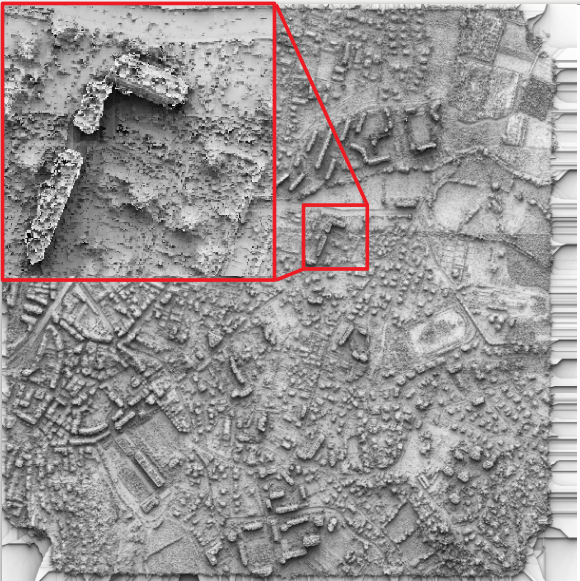
\includegraphics[width=5cm]{images/appendix4/DepthShade.png}
				%\caption{DoD$_{Pezenas\_1981}^{Co-Reg}$}
			\end{minipage}%
		}
		\caption{Comparison of precise matching on original RGB images and DSMs.}
		\label{precisematchingdepth}
	\end{center}
\end{figure*} 

